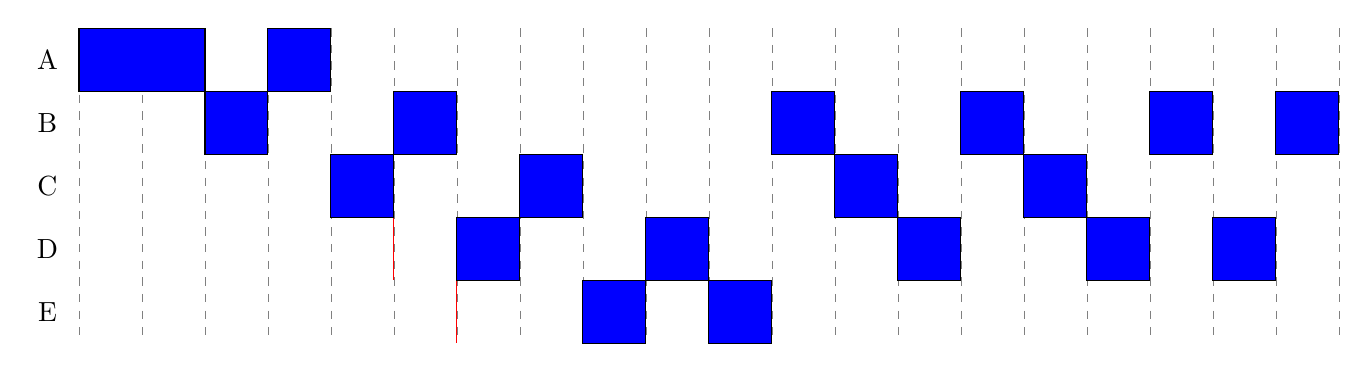
\begin{tikzpicture}[scale=.8]
   \foreach \i in {0,...,20}
   \draw[dashed, help lines] (\i,0) -- (\i,-5);

   \node (A) at (-.5,-.5) {A};
   \node (B) at (-.5,-1.5) {B};
   \node (C) at (-.5,-2.5) {C};
   \node (D) at (-.5,-3.5) {D};
   \node (E) at (-.5,-4.5) {E};

   \foreach \p in {0,...,4}
   \draw[red] (2+\p, -\p) --++ (0,-1);

   \draw[fill=blue] (0,0) rectangle (2,-1) rectangle (3,-2);
   \draw[fill=blue] (3,-1) rectangle (4,0);
   \draw[fill=blue] (4,-3) rectangle (5,-2) rectangle (6,-1);
   \draw[fill=blue] (6,-4) rectangle (7,-3) rectangle (8,-2);
   \draw[fill=blue] (8,-5) rectangle (9,-4) rectangle (10,-3);
   \draw[fill=blue] (10,-5) rectangle (11,-4);
   \draw[fill=blue] (11,-1) rectangle (12,-2) rectangle (13,-3) rectangle (14,-4);
   \draw[fill=blue] (14,-1) rectangle (15,-2) rectangle (16,-3) rectangle (17,-4);
   \draw[fill=blue] (17,-1) rectangle (18,-2);
   \draw[fill=blue] (18,-4) rectangle (19,-3) (19,-2) rectangle (20,-1);


\end{tikzpicture}

%Tt      4     20    16    19    11    //
%Tr      4     18    12    13    3     10
%Tr/Ts   4/3   18/6  12/4  13/5  3/2   2.29